\documentclass[twoside]{book}

% Packages required by doxygen
\usepackage{fixltx2e}
\usepackage{calc}
\usepackage{doxygen}
\usepackage[export]{adjustbox} % also loads graphicx
\usepackage{graphicx}
\usepackage[utf8]{inputenc}
\usepackage{makeidx}
\usepackage{multicol}
\usepackage{multirow}
\PassOptionsToPackage{warn}{textcomp}
\usepackage{textcomp}
\usepackage[nointegrals]{wasysym}
\usepackage[table]{xcolor}

% Font selection
\usepackage[T1]{fontenc}
\usepackage[scaled=.90]{helvet}
\usepackage{courier}
\usepackage{amssymb}
\usepackage{sectsty}
\renewcommand{\familydefault}{\sfdefault}
\allsectionsfont{%
  \fontseries{bc}\selectfont%
  \color{darkgray}%
}
\renewcommand{\DoxyLabelFont}{%
  \fontseries{bc}\selectfont%
  \color{darkgray}%
}
\newcommand{\+}{\discretionary{\mbox{\scriptsize$\hookleftarrow$}}{}{}}

% Page & text layout
\usepackage{geometry}
\geometry{%
  a4paper,%
  top=2.5cm,%
  bottom=2.5cm,%
  left=2.5cm,%
  right=2.5cm%
}
\tolerance=750
\hfuzz=15pt
\hbadness=750
\setlength{\emergencystretch}{15pt}
\setlength{\parindent}{0cm}
\setlength{\parskip}{3ex plus 2ex minus 2ex}
\makeatletter
\renewcommand{\paragraph}{%
  \@startsection{paragraph}{4}{0ex}{-1.0ex}{1.0ex}{%
    \normalfont\normalsize\bfseries\SS@parafont%
  }%
}
\renewcommand{\subparagraph}{%
  \@startsection{subparagraph}{5}{0ex}{-1.0ex}{1.0ex}{%
    \normalfont\normalsize\bfseries\SS@subparafont%
  }%
}
\makeatother

% Headers & footers
\usepackage{fancyhdr}
\pagestyle{fancyplain}
\fancyhead[LE]{\fancyplain{}{\bfseries\thepage}}
\fancyhead[CE]{\fancyplain{}{}}
\fancyhead[RE]{\fancyplain{}{\bfseries\leftmark}}
\fancyhead[LO]{\fancyplain{}{\bfseries\rightmark}}
\fancyhead[CO]{\fancyplain{}{}}
\fancyhead[RO]{\fancyplain{}{\bfseries\thepage}}
\fancyfoot[LE]{\fancyplain{}{}}
\fancyfoot[CE]{\fancyplain{}{}}
\fancyfoot[RE]{\fancyplain{}{\bfseries\scriptsize Generated by Doxygen }}
\fancyfoot[LO]{\fancyplain{}{\bfseries\scriptsize Generated by Doxygen }}
\fancyfoot[CO]{\fancyplain{}{}}
\fancyfoot[RO]{\fancyplain{}{}}
\renewcommand{\footrulewidth}{0.4pt}
\renewcommand{\chaptermark}[1]{%
  \markboth{#1}{}%
}
\renewcommand{\sectionmark}[1]{%
  \markright{\thesection\ #1}%
}

% Indices & bibliography
\usepackage{natbib}
\usepackage[titles]{tocloft}
\setcounter{tocdepth}{3}
\setcounter{secnumdepth}{5}
\makeindex

% Hyperlinks (required, but should be loaded last)
\usepackage{ifpdf}
\ifpdf
  \usepackage[pdftex,pagebackref=true]{hyperref}
\else
  \usepackage[ps2pdf,pagebackref=true]{hyperref}
\fi
\hypersetup{%
  colorlinks=true,%
  linkcolor=blue,%
  citecolor=blue,%
  unicode%
}

% Custom commands
\newcommand{\clearemptydoublepage}{%
  \newpage{\pagestyle{empty}\cleardoublepage}%
}

\usepackage{caption}
\captionsetup{labelsep=space,justification=centering,font={bf},singlelinecheck=off,skip=4pt,position=top}

%===== C O N T E N T S =====

\begin{document}

% Titlepage & ToC
\hypersetup{pageanchor=false,
             bookmarksnumbered=true,
             pdfencoding=unicode
            }
\pagenumbering{roman}
\begin{titlepage}
\vspace*{7cm}
\begin{center}%
{\Large My Project }\\
\vspace*{1cm}
{\large Generated by Doxygen 1.8.11}\\
\end{center}
\end{titlepage}
\clearemptydoublepage
\tableofcontents
\clearemptydoublepage
\pagenumbering{arabic}
\hypersetup{pageanchor=true}

%--- Begin generated contents ---
\chapter{File Index}
\section{File List}
Here is a list of all files with brief descriptions\+:\begin{DoxyCompactList}
\item\contentsline{section}{\hyperlink{Lab1_8c}{Lab1.\+c} }{\pageref{Lab1_8c}}{}
\end{DoxyCompactList}

\chapter{File Documentation}
\hypertarget{UnionAndInstersection_8c}{}\section{Union\+And\+Instersection.\+c File Reference}
\label{UnionAndInstersection_8c}\index{Union\+And\+Instersection.\+c@{Union\+And\+Instersection.\+c}}
{\ttfamily \#include $<$stdio.\+h$>$}\\*
Include dependency graph for Union\+And\+Instersection.\+c\+:
\nopagebreak
\begin{figure}[H]
\begin{center}
\leavevmode
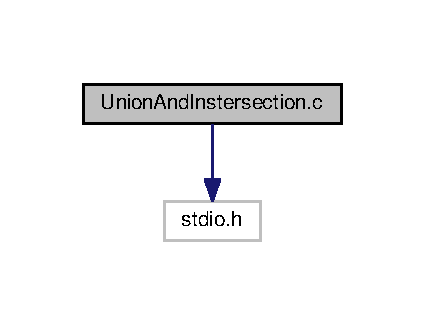
\includegraphics[width=204pt]{UnionAndInstersection_8c__incl}
\end{center}
\end{figure}
\subsection*{Macros}
\begin{DoxyCompactItemize}
\item 
\#define \hyperlink{UnionAndInstersection_8c_a70ed59adcb4159ac551058053e649640}{S\+I\+ZE}~5
\end{DoxyCompactItemize}
\subsection*{Functions}
\begin{DoxyCompactItemize}
\item 
void \hyperlink{UnionAndInstersection_8c_a410b2addcc7a3a00210eb21d9d3b10b4}{get\+\_\+value} (int arr\mbox{[}$\,$\mbox{]})
\item 
void \hyperlink{UnionAndInstersection_8c_a91ca11cd52ff629eb9c904beec08878f}{print\+\_\+value} (int arr\mbox{[}$\,$\mbox{]}, int n)
\item 
void \hyperlink{UnionAndInstersection_8c_a5b42cb5c09d50e423862dd90755c5412}{function\+\_\+sort} (int arr\mbox{[}$\,$\mbox{]})
\item 
int \hyperlink{UnionAndInstersection_8c_a75c51101c470aa6bff490a55b0165bab}{find\+\_\+intersection} (int array1\mbox{[}$\,$\mbox{]}, int array2\mbox{[}$\,$\mbox{]}, int intersection\+\_\+array\mbox{[}$\,$\mbox{]})
\item 
int \hyperlink{UnionAndInstersection_8c_a4ab04fd44a096d59ca0bb9bef8af739d}{find\+\_\+union} (int array1\mbox{[}$\,$\mbox{]}, int array2\mbox{[}$\,$\mbox{]}, int union\+\_\+array\mbox{[}$\,$\mbox{]})
\item 
void \hyperlink{UnionAndInstersection_8c_acdef7a1fd863a6d3770c1268cb06add3}{main} ()
\end{DoxyCompactItemize}


\subsection{Macro Definition Documentation}
\index{Union\+And\+Instersection.\+c@{Union\+And\+Instersection.\+c}!S\+I\+ZE@{S\+I\+ZE}}
\index{S\+I\+ZE@{S\+I\+ZE}!Union\+And\+Instersection.\+c@{Union\+And\+Instersection.\+c}}
\subsubsection[{\texorpdfstring{S\+I\+ZE}{SIZE}}]{\setlength{\rightskip}{0pt plus 5cm}\#define S\+I\+ZE~5}\hypertarget{UnionAndInstersection_8c_a70ed59adcb4159ac551058053e649640}{}\label{UnionAndInstersection_8c_a70ed59adcb4159ac551058053e649640}


\subsection{Function Documentation}
\index{Union\+And\+Instersection.\+c@{Union\+And\+Instersection.\+c}!find\+\_\+intersection@{find\+\_\+intersection}}
\index{find\+\_\+intersection@{find\+\_\+intersection}!Union\+And\+Instersection.\+c@{Union\+And\+Instersection.\+c}}
\subsubsection[{\texorpdfstring{find\+\_\+intersection(int array1[], int array2[], int intersection\+\_\+array[])}{find_intersection(int array1[], int array2[], int intersection_array[])}}]{\setlength{\rightskip}{0pt plus 5cm}int find\+\_\+intersection (
\begin{DoxyParamCaption}
\item[{int}]{array1\mbox{[}$\,$\mbox{]}, }
\item[{int}]{array2\mbox{[}$\,$\mbox{]}, }
\item[{int}]{intersection\+\_\+array\mbox{[}$\,$\mbox{]}}
\end{DoxyParamCaption}
)}\hypertarget{UnionAndInstersection_8c_a75c51101c470aa6bff490a55b0165bab}{}\label{UnionAndInstersection_8c_a75c51101c470aa6bff490a55b0165bab}

\begin{DoxyCode}
98 \{
99     \textcolor{keywordtype}{int} i = 0, j = 0, k = 0;
100     \textcolor{keywordflow}{while} ((i < \hyperlink{UnionAndInstersection_8c_a70ed59adcb4159ac551058053e649640}{SIZE}) && (j < \hyperlink{UnionAndInstersection_8c_a70ed59adcb4159ac551058053e649640}{SIZE}))
101     \{
102         \textcolor{keywordflow}{if} (array1[i] < array2[j])
103         \{
104             i++;
105         \}
106         \textcolor{keywordflow}{else} \textcolor{keywordflow}{if} (array1[i] > array2[j])
107         \{
108             j++;
109         \}
110         \textcolor{keywordflow}{else}
111         \{
112             intersection\_array[k] = array1[i];
113             i++;
114             j++;
115             k++;
116         \}
117     \}
118     \textcolor{keywordflow}{return}(k);
119 \}
\end{DoxyCode}
\index{Union\+And\+Instersection.\+c@{Union\+And\+Instersection.\+c}!find\+\_\+union@{find\+\_\+union}}
\index{find\+\_\+union@{find\+\_\+union}!Union\+And\+Instersection.\+c@{Union\+And\+Instersection.\+c}}
\subsubsection[{\texorpdfstring{find\+\_\+union(int array1[], int array2[], int union\+\_\+array[])}{find_union(int array1[], int array2[], int union_array[])}}]{\setlength{\rightskip}{0pt plus 5cm}int find\+\_\+union (
\begin{DoxyParamCaption}
\item[{int}]{array1\mbox{[}$\,$\mbox{]}, }
\item[{int}]{array2\mbox{[}$\,$\mbox{]}, }
\item[{int}]{union\+\_\+array\mbox{[}$\,$\mbox{]}}
\end{DoxyParamCaption}
)}\hypertarget{UnionAndInstersection_8c_a4ab04fd44a096d59ca0bb9bef8af739d}{}\label{UnionAndInstersection_8c_a4ab04fd44a096d59ca0bb9bef8af739d}

\begin{DoxyCode}
122 \{
123     \textcolor{keywordtype}{int} i = 0, j = 0, k = 0;
124     \textcolor{keywordflow}{while} ((i < \hyperlink{UnionAndInstersection_8c_a70ed59adcb4159ac551058053e649640}{SIZE}) && (j < \hyperlink{UnionAndInstersection_8c_a70ed59adcb4159ac551058053e649640}{SIZE}))
125     \{
126         \textcolor{keywordflow}{if} (array1[i] < array2[j])
127         \{
128             union\_array[k] = array1[i];
129             i++;
130             k++;
131         \}
132         \textcolor{keywordflow}{else} \textcolor{keywordflow}{if} (array1[i] > array2[j])
133         \{
134             union\_array[k] = array2[j];
135             j++;
136             k++;
137         \}
138         \textcolor{keywordflow}{else}
139         \{
140             union\_array[k] = array1[i];
141             i++;
142             j++;
143             k++;
144         \}
145     \}
146     \textcolor{keywordflow}{if} (i == \hyperlink{UnionAndInstersection_8c_a70ed59adcb4159ac551058053e649640}{SIZE})
147     \{
148         \textcolor{keywordflow}{while} (j < \hyperlink{UnionAndInstersection_8c_a70ed59adcb4159ac551058053e649640}{SIZE})
149         \{
150             union\_array[k] = array2[j];
151             j++;
152             k++;
153         \}
154     \}
155     \textcolor{keywordflow}{else}
156     \{
157         \textcolor{keywordflow}{while} (i < \hyperlink{UnionAndInstersection_8c_a70ed59adcb4159ac551058053e649640}{SIZE})
158         \{
159             union\_array[k] = array1[i];
160             i++;
161             k++;
162         \}
163     \}
164     \textcolor{keywordflow}{return}(k);
165 \}
\end{DoxyCode}
\index{Union\+And\+Instersection.\+c@{Union\+And\+Instersection.\+c}!function\+\_\+sort@{function\+\_\+sort}}
\index{function\+\_\+sort@{function\+\_\+sort}!Union\+And\+Instersection.\+c@{Union\+And\+Instersection.\+c}}
\subsubsection[{\texorpdfstring{function\+\_\+sort(int arr[])}{function_sort(int arr[])}}]{\setlength{\rightskip}{0pt plus 5cm}void function\+\_\+sort (
\begin{DoxyParamCaption}
\item[{int}]{arr\mbox{[}$\,$\mbox{]}}
\end{DoxyParamCaption}
)}\hypertarget{UnionAndInstersection_8c_a5b42cb5c09d50e423862dd90755c5412}{}\label{UnionAndInstersection_8c_a5b42cb5c09d50e423862dd90755c5412}

\begin{DoxyCode}
74 \{
75     \textcolor{keywordtype}{int} i, j, temp, swapping;
76  
77     \textcolor{keywordflow}{for} (i = 1; i < \hyperlink{UnionAndInstersection_8c_a70ed59adcb4159ac551058053e649640}{SIZE}; i++)
78     \{
79         swapping = 0;
80         \textcolor{keywordflow}{for} (j = 0; j < SIZE-i; j++)
81         \{
82             \textcolor{keywordflow}{if} (arr[j] > arr[j+1])
83             \{
84                 temp = arr[j];
85                 arr[j] = arr[j + 1];
86                 arr[j + 1] = temp;
87                 swapping = 1;
88             \}
89         \}
90         \textcolor{keywordflow}{if} (swapping == 0)
91         \{
92             \textcolor{keywordflow}{break};
93         \}
94     \}
95 \}
\end{DoxyCode}
\index{Union\+And\+Instersection.\+c@{Union\+And\+Instersection.\+c}!get\+\_\+value@{get\+\_\+value}}
\index{get\+\_\+value@{get\+\_\+value}!Union\+And\+Instersection.\+c@{Union\+And\+Instersection.\+c}}
\subsubsection[{\texorpdfstring{get\+\_\+value(int arr[])}{get_value(int arr[])}}]{\setlength{\rightskip}{0pt plus 5cm}void get\+\_\+value (
\begin{DoxyParamCaption}
\item[{int}]{arr\mbox{[}$\,$\mbox{]}}
\end{DoxyParamCaption}
)}\hypertarget{UnionAndInstersection_8c_a410b2addcc7a3a00210eb21d9d3b10b4}{}\label{UnionAndInstersection_8c_a410b2addcc7a3a00210eb21d9d3b10b4}

\begin{DoxyCode}
52 \{
53     \textcolor{keywordtype}{int} i, j;
54     \textcolor{keywordflow}{for} (i = 0; i < \hyperlink{UnionAndInstersection_8c_a70ed59adcb4159ac551058053e649640}{SIZE}; i++)
55     \{
56         j = i + 1;
57         printf(\textcolor{stringliteral}{"\(\backslash\)n Enter element %d: "}, j);
58         scanf(\textcolor{stringliteral}{"%d"}, &arr[i]);
59     \}
60 \}
\end{DoxyCode}
\index{Union\+And\+Instersection.\+c@{Union\+And\+Instersection.\+c}!main@{main}}
\index{main@{main}!Union\+And\+Instersection.\+c@{Union\+And\+Instersection.\+c}}
\subsubsection[{\texorpdfstring{main()}{main()}}]{\setlength{\rightskip}{0pt plus 5cm}void main (
\begin{DoxyParamCaption}
{}
\end{DoxyParamCaption}
)}\hypertarget{UnionAndInstersection_8c_acdef7a1fd863a6d3770c1268cb06add3}{}\label{UnionAndInstersection_8c_acdef7a1fd863a6d3770c1268cb06add3}

\begin{DoxyCode}
14 \{
15     \textcolor{keywordtype}{int} array1[\hyperlink{UnionAndInstersection_8c_a70ed59adcb4159ac551058053e649640}{SIZE}], array2[\hyperlink{UnionAndInstersection_8c_a70ed59adcb4159ac551058053e649640}{SIZE}], intersection\_array[\hyperlink{UnionAndInstersection_8c_a70ed59adcb4159ac551058053e649640}{SIZE}], union\_array[
      \hyperlink{UnionAndInstersection_8c_a70ed59adcb4159ac551058053e649640}{SIZE}*2];
16     \textcolor{keywordtype}{int} num\_elements;
17  
18     \textcolor{comment}{//input elements of Array1}
19     printf(\textcolor{stringliteral}{"\(\backslash\)n Enter the elements of Array 1: n"});
20     \hyperlink{UnionAndInstersection_8c_a410b2addcc7a3a00210eb21d9d3b10b4}{get\_value}(array1);
21     printf(\textcolor{stringliteral}{"\(\backslash\)n\(\backslash\)n Elements of Array 1: "});
22     \hyperlink{UnionAndInstersection_8c_a91ca11cd52ff629eb9c904beec08878f}{print\_value}(array1, \hyperlink{UnionAndInstersection_8c_a70ed59adcb4159ac551058053e649640}{SIZE});
23  
24     \textcolor{comment}{//Sort array 1}
25     \hyperlink{UnionAndInstersection_8c_a5b42cb5c09d50e423862dd90755c5412}{function\_sort}(array1);
26     printf(\textcolor{stringliteral}{"nnSorted elements of Array 1: "});
27     \hyperlink{UnionAndInstersection_8c_a91ca11cd52ff629eb9c904beec08878f}{print\_value}(array1, \hyperlink{UnionAndInstersection_8c_a70ed59adcb4159ac551058053e649640}{SIZE});
28  
29     \textcolor{comment}{//input elements of Array2}
30     printf(\textcolor{stringliteral}{"nnEnter the elements of Array 2: n"});
31     \hyperlink{UnionAndInstersection_8c_a410b2addcc7a3a00210eb21d9d3b10b4}{get\_value}(array2);
32     printf(\textcolor{stringliteral}{"\(\backslash\)n\(\backslash\)n Elements of Array 2: "});
33     \hyperlink{UnionAndInstersection_8c_a91ca11cd52ff629eb9c904beec08878f}{print\_value}(array2, \hyperlink{UnionAndInstersection_8c_a70ed59adcb4159ac551058053e649640}{SIZE});
34  
35     \textcolor{comment}{//Sort array 2}
36     \hyperlink{UnionAndInstersection_8c_a5b42cb5c09d50e423862dd90755c5412}{function\_sort}(array2);
37     printf(\textcolor{stringliteral}{"\(\backslash\)n\(\backslash\)nSorted elements of Array 2: "});
38     \hyperlink{UnionAndInstersection_8c_a91ca11cd52ff629eb9c904beec08878f}{print\_value}(array2, \hyperlink{UnionAndInstersection_8c_a70ed59adcb4159ac551058053e649640}{SIZE});
39  
40     \textcolor{comment}{//Find Intersection}
41     num\_elements = \hyperlink{UnionAndInstersection_8c_a75c51101c470aa6bff490a55b0165bab}{find\_intersection}(array1, array2, intersection\_array);
42     printf(\textcolor{stringliteral}{"\(\backslash\)n\(\backslash\)n Intersection is: "});
43     \hyperlink{UnionAndInstersection_8c_a91ca11cd52ff629eb9c904beec08878f}{print\_value}(intersection\_array, num\_elements);
44  
45     \textcolor{comment}{//Find Union}
46     num\_elements = \hyperlink{UnionAndInstersection_8c_a4ab04fd44a096d59ca0bb9bef8af739d}{find\_union}(array1, array2, union\_array);
47     printf(\textcolor{stringliteral}{"\(\backslash\)n\(\backslash\)n Union is: "});
48     \hyperlink{UnionAndInstersection_8c_a91ca11cd52ff629eb9c904beec08878f}{print\_value}(union\_array, num\_elements);
49 \}
\end{DoxyCode}


Here is the call graph for this function\+:
\nopagebreak
\begin{figure}[H]
\begin{center}
\leavevmode
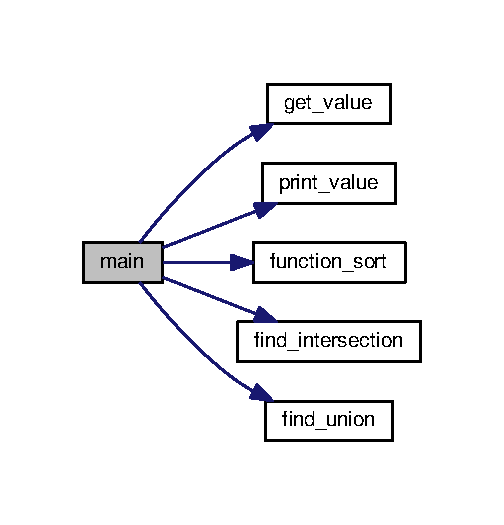
\includegraphics[width=242pt]{UnionAndInstersection_8c_acdef7a1fd863a6d3770c1268cb06add3_cgraph}
\end{center}
\end{figure}


\index{Union\+And\+Instersection.\+c@{Union\+And\+Instersection.\+c}!print\+\_\+value@{print\+\_\+value}}
\index{print\+\_\+value@{print\+\_\+value}!Union\+And\+Instersection.\+c@{Union\+And\+Instersection.\+c}}
\subsubsection[{\texorpdfstring{print\+\_\+value(int arr[], int n)}{print_value(int arr[], int n)}}]{\setlength{\rightskip}{0pt plus 5cm}void print\+\_\+value (
\begin{DoxyParamCaption}
\item[{int}]{arr\mbox{[}$\,$\mbox{]}, }
\item[{int}]{n}
\end{DoxyParamCaption}
)}\hypertarget{UnionAndInstersection_8c_a91ca11cd52ff629eb9c904beec08878f}{}\label{UnionAndInstersection_8c_a91ca11cd52ff629eb9c904beec08878f}

\begin{DoxyCode}
63 \{
64     \textcolor{keywordtype}{int} i;
65     printf(\textcolor{stringliteral}{"\{ "});
66     \textcolor{keywordflow}{for} (i = 0; i < n; i++)
67     \{
68         printf(\textcolor{stringliteral}{"%d "}, arr[i]);
69     \}
70     printf(\textcolor{stringliteral}{"\}"});
71 \}
\end{DoxyCode}

%--- End generated contents ---

% Index
\backmatter
\newpage
\phantomsection
\clearemptydoublepage
\addcontentsline{toc}{chapter}{Index}
\printindex

\end{document}
